%%%%%%%%%%%%%%%%%%%%%%%%%%%%%%%%%%%%%%%%%%%%%%%%%%%%%%%%%%%%%%%%%%%%
%% appendix1.tex
%% NOVA thesis document file
%%
%% Appendix with architectural layers flowcharts %% that were too small on the main text. 
%%%%%%%%%%%%%%%%%%%%%%%%%%%%%%%%%%%%%%%%%%%%%%%%%%%%%%%%%%%%%%%%%%%%
\chapter{Architectural Layers Flowcharts}
\label{app:architectural_layers_flowcharts}

This appendix presents the camera spatial processing flowcharts in bigger scale.

\begin{figure}[htbp]
	\centering
	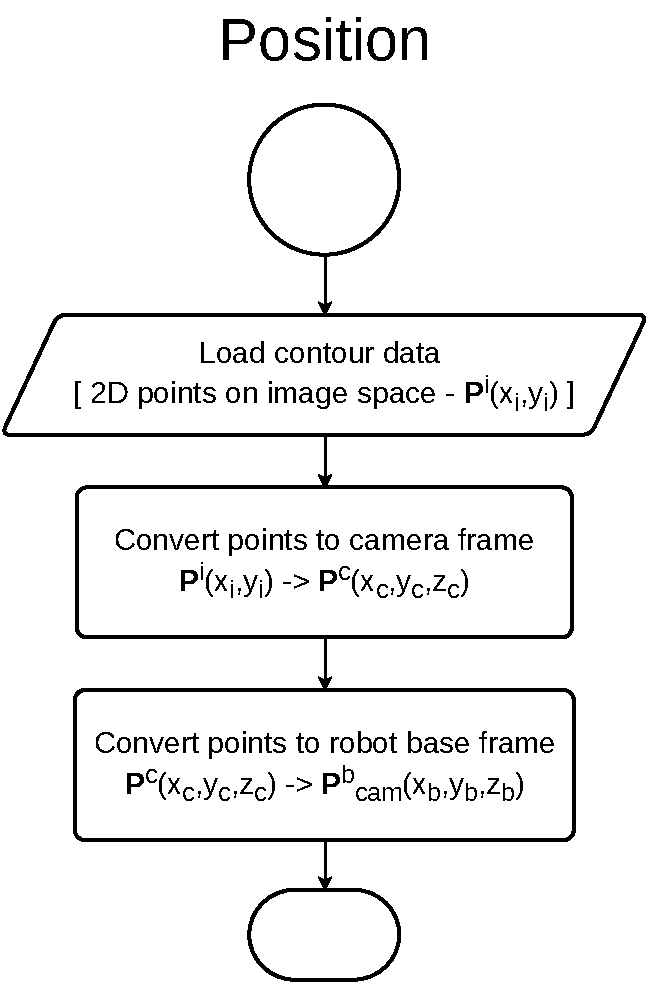
\includegraphics[height=12cm]{system_architecture_layer_camera_spatial_data_flowchart_position}
	\caption[Camera spatial data processing flowchart for obtaining wound position.]{Camera spatial data processing flowchart for obtaining wound position.}
	\label{fig:system_architecture_layer_camera_spatial_data_flowchart_position}
\end{figure}

\begin{figure}[htbp]
	\centering
	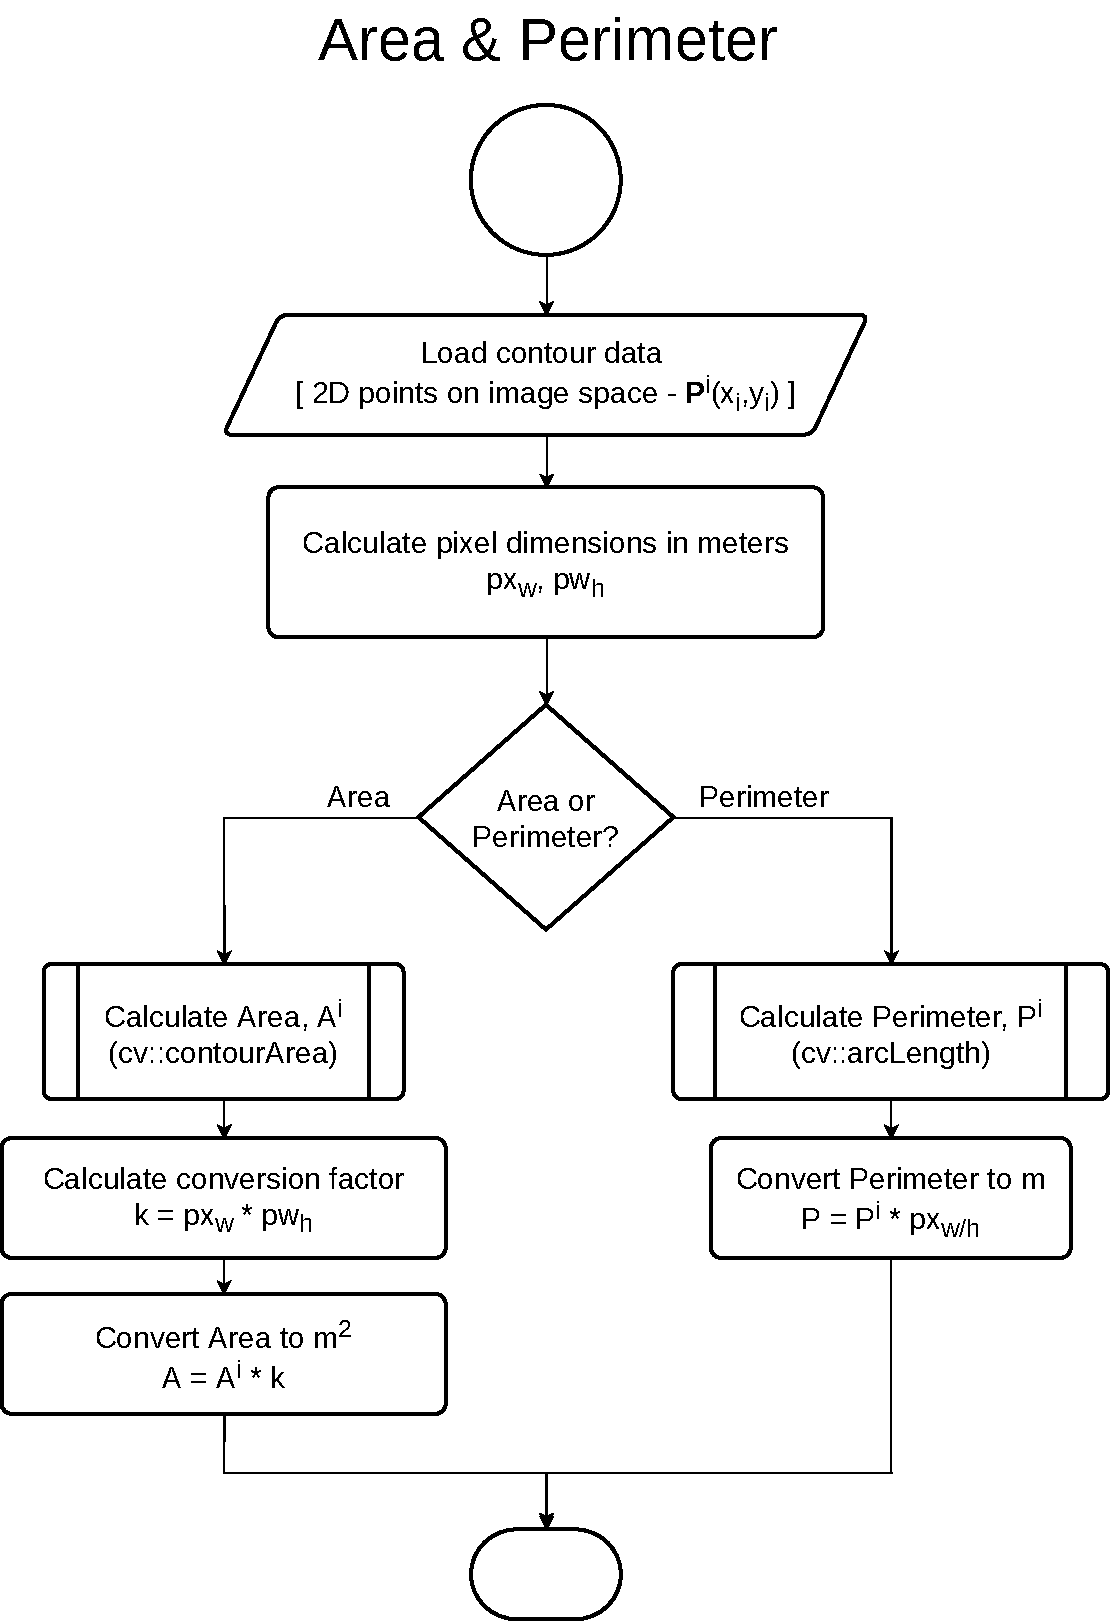
\includegraphics[height=18cm]{system_architecture_layer_camera_spatial_data_flowchart_area_perimeter}
	\caption[Camera spatial data processing flowchart to calculate the wound area and perimeter.]{Camera spatial data processing flowchart to calculate the wound area and perimeter.}
	\label{fig:system_architecture_layer_camera_spatial_data_flowchart_area_perimeter}
\end{figure}

\begin{figure}[htbp]
	\centering
	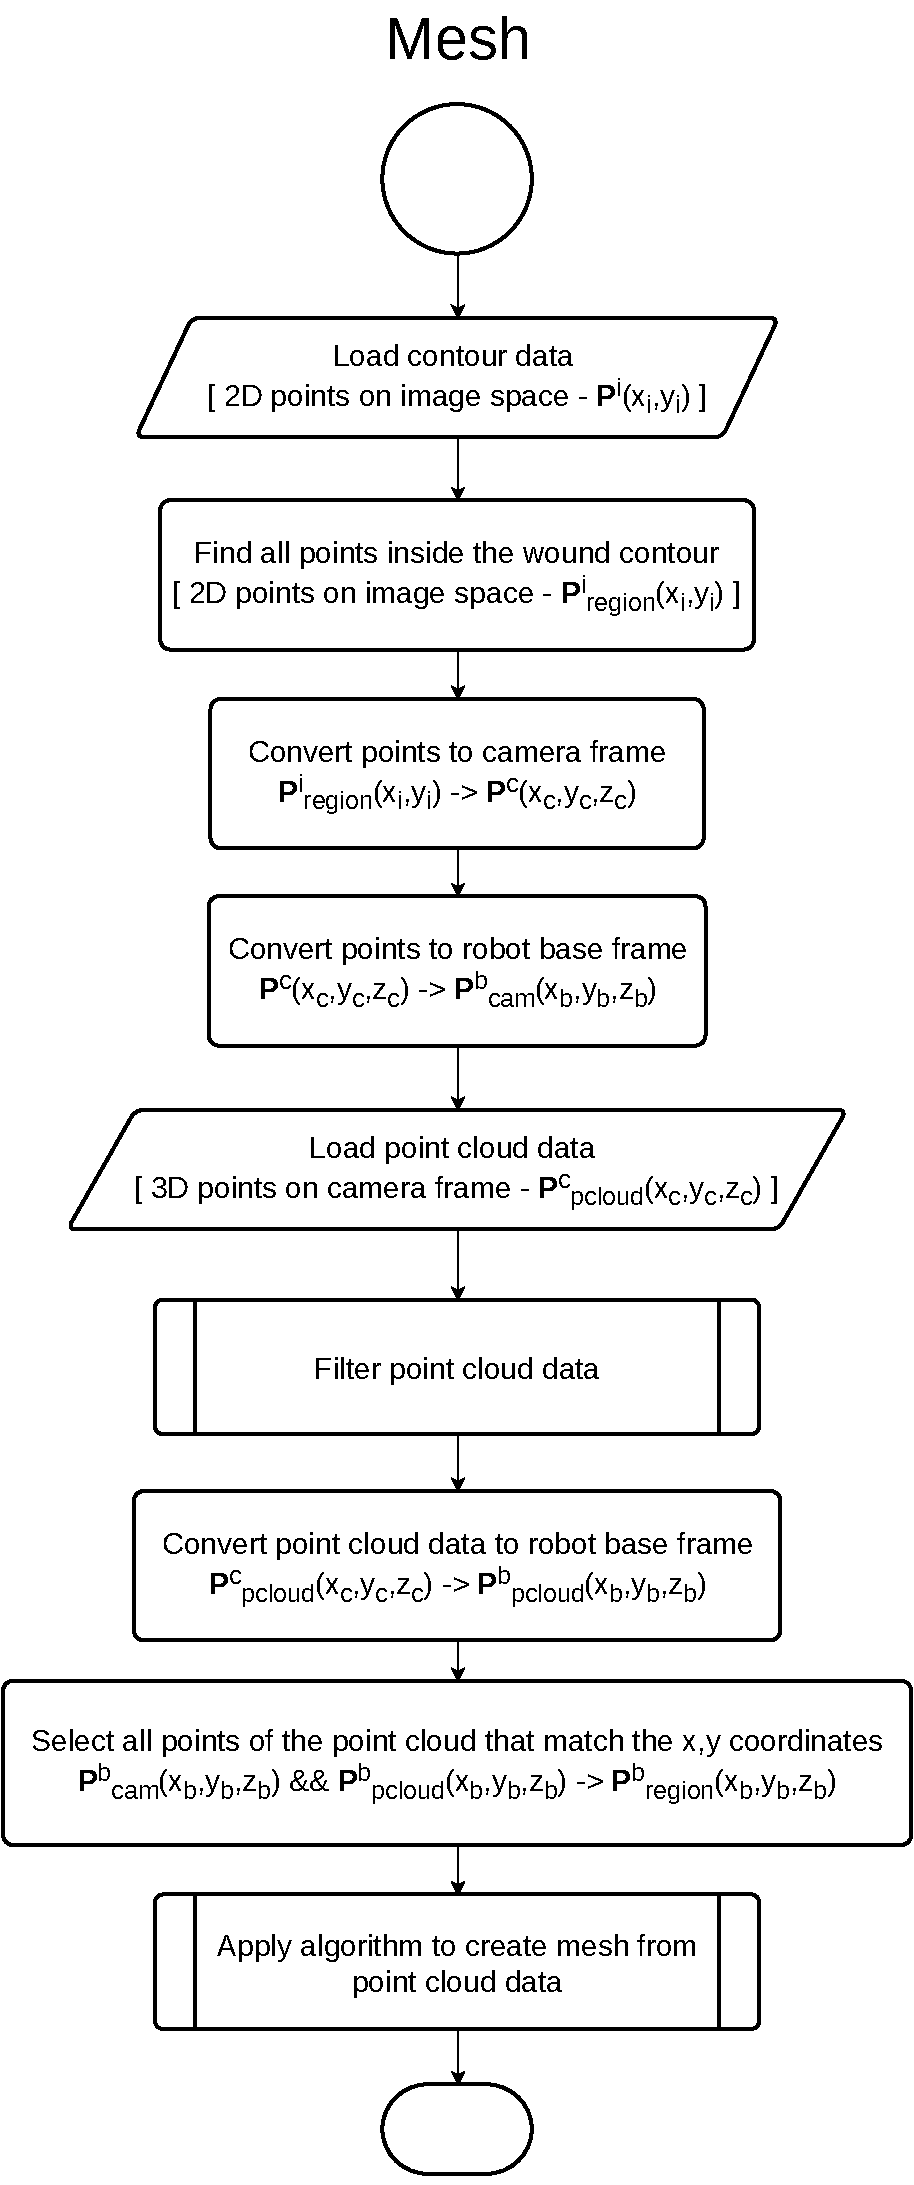
\includegraphics[height=21cm]{system_architecture_layer_camera_spatial_data_flowchart_mesh}
	\caption[Camera spatial data processing mesh generation flowchart.]{Camera spatial data processing mesh generation flowchart.}
	\label{fig:system_architecture_layer_camera_spatial_data_flowchart_mesh}
\end{figure}